\section{Application Implementation}
The application used for the study used an earlier version of the Mobility Features Package which required the programmer to write a lot of code to compute the features. This section will provide source code examples of how the application should be implemented with the latest version of the package. The functionality of the study app has not changed but the source code for the application related to feature computation takes up much fewer lines.

\subsection{Architecture Overview}
To provide a high-level overview of the different classs which make up the study application, a high level class diagram is displayed in Figure \ref{fig:app-class-diagram}. The MobilityStudy class is responsible for managing the application state but does not do much outside of this since the application state management required is minimal. The Main Screen class is spawned from the MobilityStudy class and runs an instance of the AppProcessor class. The AppProcessor instance is responsible for a multitude of tasks, such as asking for permissions, collection location data, and computing features. Storing and loading from the disk is done through the FileManager class which includes LocationSamples Stops, Moves, MobilityContexts, and diary answers. This class is also responsible for uploading the stored data to a Firebase server.

\begin{figure}
    \centering
    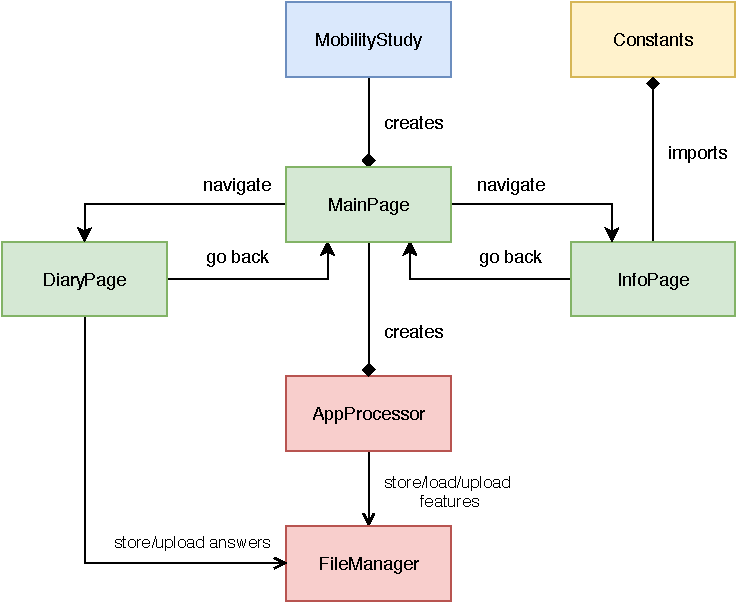
\includegraphics[width=0.7\textwidth]{images/diagrams/app-diagram.pdf}
    \caption{class diagram for the study application displaying the different building blocks and the interactions between them}
    \label{fig:app-class-diagram}
\end{figure}

\subsection{Custom Location Plugin}
For collecting Location Samples, a custom version of the \textit{Geolocator}\footnote{\url{https://pub.dev/packages/geolocator}} plugin was developed for the purpose of this package to achieve reliable background location streaming. The current implementation of \textit{Geolocator} was missing a flag in the \textit{Objective-C} implementation for iOS, which allows the app to continue streaming location data while the app is minimized. The flag for background updates has to be set for an instance of a Location Manager which is the access to the Location API:

\begin{minted}{dart}
    _locationManager.allowsBackgroundLocationUpdates = YES;
\end{minted}

If this flag is not set to 'YES' (i.e. True), the location stream will die shortly after the application is minimized. It is important to note that this plugin is not part of the Mobility Features Package, but is needed for high-frequency background location tracking. A Github issue was created\footnote{\url{https://github.com/Baseflow/flutter-geolocator/issues/390}} and the features were accepted and merged into a development branch for the GeoLocator plugin. The functionality is however not public as of yet, and the custom plugin was, therefore, necessary to use when developing the application. 

\subsection{Collecting Location Samples}
The custom Geolocator plugin was used to set up a stream of location data. The DTO of the plugin called Position, and contains latitude, longitude, and timestamp, in addition to other GPS information. The stream is set up with a subscription using a call-back method that is invoked every time a Position object is generated by the stream. 

\begin{minted}{dart}
await _geoLocator.isLocationServiceEnabled().then((response) {
  if (response) {
    streamingLocation = true;
    _subscription = _geoLocator.getPositionStream(options).listen(_onData);
  } else {
    print('Location service not enabled');
  }
});
\end{minted}

This call-back method is the \verb|_onData| method which is responsible for saving the collected data. It does so by first converting the Position DTO object into a LocationSample DTO object, and then adding it to a buffer. This buffer is implemented as a List of LocationSamples and when the number of samples in this buffer exceeds 100, the content of the buffer will be stored to disk via the \verb|ContextGenerator|. Afterward, the buffer is emptied, and the process starts anew. 

\begin{figure}
    \centering
    \begin{minted}{dart}
      void _onData(Position x) async {
        GeoPosition gp = GeoPosition(x.latitude, x.longitude);
        LocationSample sample = LocationSample(gp, x.timestamp);
        _buffer.add(sample);

        if (_buffer.length >= BUFFER_SIZE) {
          /// Save buffer locally, empty it,  then upload data
          await ContextGenerator.saveSamples(_buffer);
          _buffer = [];
          await FileManager().uploadSamples(uuid);
    
          /// If enough data has been collected, evaluate features
          numberOfBuffers++;
          if (numberOfBuffers >= 5) {
            numberOfBuffers = 0;
    
            /// Offload computation to background, do not await
            _computeFeaturesAsync();
          }
        }
      }
    \end{minted}
    \caption{The \textit{\_onData} method responsible for handling incoming Location DTOs}
    \label{fig:ondata-method}
\end{figure}


\subsection{Firebase Services}
Firebase file storage was used to host all the data generated by the study application. File storage hosted on a centralized server made it easy to oversee the study and check in on users to see if they remembered to provide answers and track their location. \\

Additionally, the Firebase Cloud Messaging (FCM) service was set up such that push notifications could be delivered to the participants' phones via the application, to remind them to fill out the diary. Push notifications are sent out from a centralized server and can be edited at any time without access to the physical phones. In was sometimes useful to send out extra notifications to specific users if they forgot to fill out many days in a row.

\subsection{Computing Features and Async Calls}
Every time the buffer has been been filled and stored to the disk 5 times, features are computed. This was done to demonstrate the real-time capability of the Mobility Features Package, i.e. computing features multiple times a day on an incomplete dataset. Features were also computed when the user navigated to the DiaryPage, such that they are generated close to answers being given. This however did not work if the DiaryPage was opened through a notifiation, unfortunately.\\

Flutter supports multi-threading, which means the main thread runs the user interface, and background threads can be spawned in order to perform other computations in the background. If heavy computation is done in the main thread, the user would experience a frozen UI while computation takes place. This is due to the main thread running the computations needed to make the UI able to respond to input and update itself. In the study app there was no responsive UI, but in a real-world application the UI should not freeze due to the feature calculation. Dart threads are referred to as \textit{isolates} which communicate using a \textit{SendPort} and a \textit{ReceivePort}. These ports can be used to transfer objects between threads, such that the main thread can request a background thread to calculate the features, and the background thread will then send back a \textit{MobilityContext} object once finished. 

\begin{minted}{dart}
Future<MobilityContext> _computeFeaturesAsync() async {
  ReceivePort receivePort = ReceivePort();
  await Isolate.spawn(_asyncComputation, receivePort.sendPort);
  SendPort sendPort = await receivePort.first;

  MobilityContext mobilityContext = await _relay(sendPort);
  return mobilityContext;
}
\end{minted}

The \verb|_relay| method works as an interface between the \verb|_computeFeaturesAsync| method which runs on the UI thread and the static method \verb|_asyncComputation| which runs on the background thread and simply relays messages between the two threads.

\begin{minted}{dart}
Future _relay(SendPort sendPort) {
  ReceivePort receivePort = ReceivePort();
  sendPort.send([receivePort.sendPort]);
  return receivePort.first;
}
\end{minted}

Lastly, the \verb|_asyncComputation| method is static which is due to the computation being done in a background thread. If the objects contained within the \textit{AppProcessor} instance, running in the main thread, were to change their state while computation was ongoing in the background thread, then the results of the computation becomes non-deterministic. Therefore the objects used in the background computation cannot change their state outside the background thread. 

\begin{minted}{dart}
static void _asyncComputation(SendPort sendPort) async {
  ReceivePort receivePort = ReceivePort();
  sendPort.send(receivePort.sendPort);
  List args = await receivePort.first;
  SendPort replyPort = args[0];

  MobilityContext context =
      await ContextGenerator.generate(usePriorContexts: true);

  replyPort.send(context);
}
\end{minted}

